\documentclass{article}
\usepackage{graphicx}
\usepackage{amsmath}
\usepackage{booktabs}
\usepackage{geometry}
\geometry{a4paper, margin=1in}

\title{Matrix Sort with CUDA}
\author{Mohammadreza Naziri}
\date{40030505}

\begin{document}
\maketitle

\section{Finding the Best Block Size for System}

CUDA programs can be optimized by carefully choosing the block size (number of threads per block). I experimented with block sizes ranging from 8 to 1024 and found that a block size of 64 threads provided the best performance, even though the GPU occupancy was not at its maximum. As we try to achieve more occupancy we must increase the block size and this will lead us to lose Zero-Time-Context-Switch so the time will increase too.

\subsection{Explanation of Occupancy:}

Occupancy refers to the ratio of active warps to the maximum number of warps supported on a Streaming Multiprocessor (SM). While high occupancy is often desirable, it is not always directly correlated with peak performance. Factors like memory access patterns, computational intensity, and register usage can have a more significant impact.



\begin{figure}[h!]
    \centering
    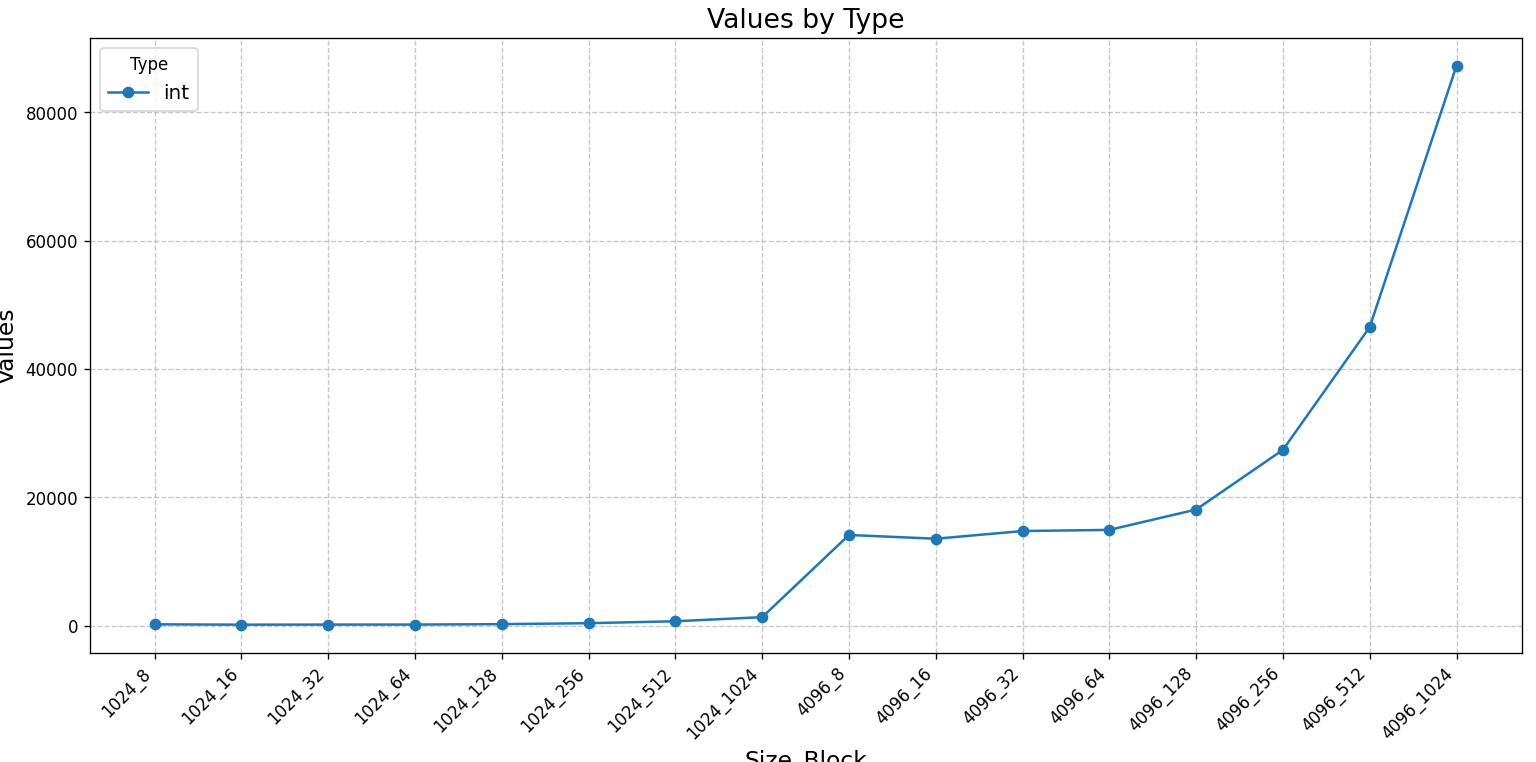
\includegraphics[width=0.8\textwidth]{1.png}
    \caption{Block Size comparison}
\end{figure}

\begin{table}[h!]
    \centering
    \begin{tabular}{@{}ccc@{}}
        \toprule
        Block Size & Occupancy (\%) & Block Number \\
        \midrule
        8 & 11.05 & 128 \\
        16 & 5.58 & 64 \\
        32 & 2.86 & 32 \\
        64 & 4.16 & 16 \\
        128 & 8.33 & 8 \\
        256 & 16.66 & 4 \\
        512 & 33.09 & 2 \\
        1024 & 66.03 & 1 \\
        \bottomrule
    \end{tabular}
    \caption{Occupancy and Block size for 1024*1024 int matrix.}
    \label{tab:block_size}
\end{table}


\section{Sequential vs Parallel (CUDA) Algorithm}

My comparison of sequential and parallel algorithms (using CUDA) reveals the significant performance improvement achieved through parallelism.

\subsection{Pipeline and Parallel Execution:}

Explain how CUDA exploits massive parallelism by dividing the workload among thousands of threads running concurrently. In contrast, a sequential algorithm processes one element at a time, leading to slower execution times.

\subsection{Conclusion:}

Discuss the scenarios where parallelism provides the most benefit, emphasizing the role of GPU’s pipeline in maximizing throughput.
\begin{figure}[h!]
    \centering
    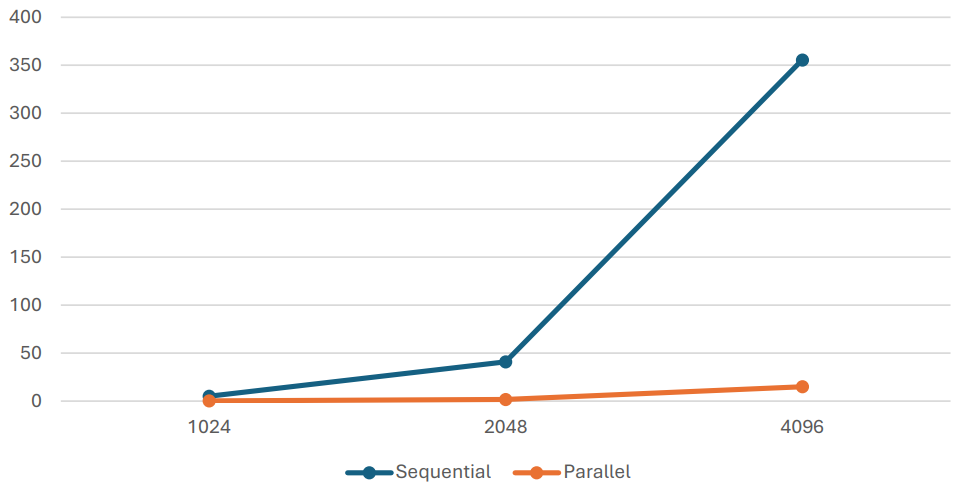
\includegraphics[width=0.8\textwidth]{2.png}
\end{figure}


\section{Comparison of Bubble Sort and Odd-Even Sort in CUDA}
I evaluated two sorting algorithms in CUDA—bubble sort and odd-even sort—and have a plot that compares their performance.


\begin{figure}[h!]
    \centering
    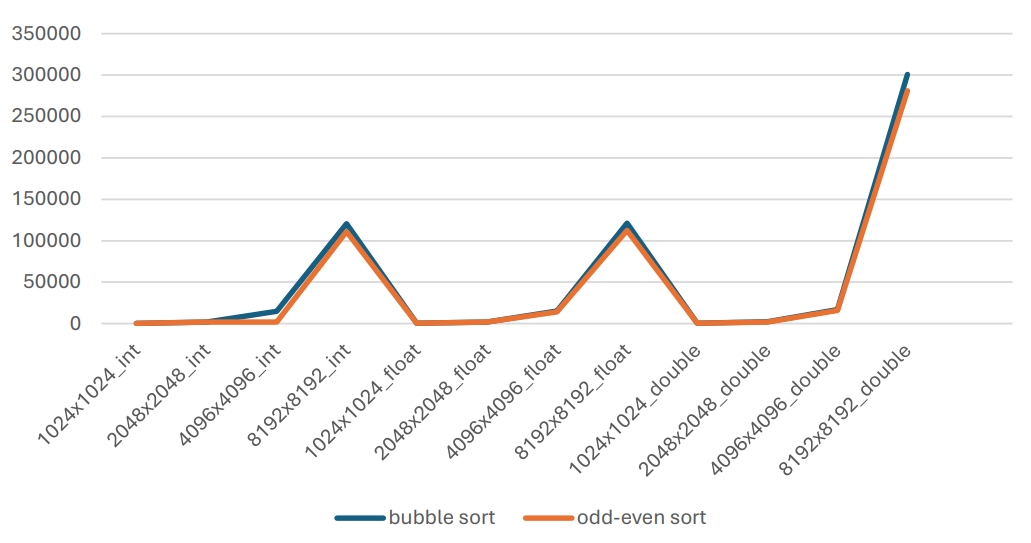
\includegraphics[width=0.8\textwidth]{3.png}
\end{figure}



\section{Running the Code for Different Data Types and Sizes}

I tested the sorting algorithms with integer, float, and double data types, as well as various array sizes (1024,2048,4096,8192).

\subsection{Effect of Data Types:}

The size of the data type affects performance. For example, double-precision computations may take longer due to increased memory bandwidth and computational requirements.

\subsection{Effect of Input Size:}

Performance scales with array size. Bottlenecks or inefficiencies observed for larger inputs, such as memory access overheads or synchronization delays.


\begin{figure}[h!]
    \centering
    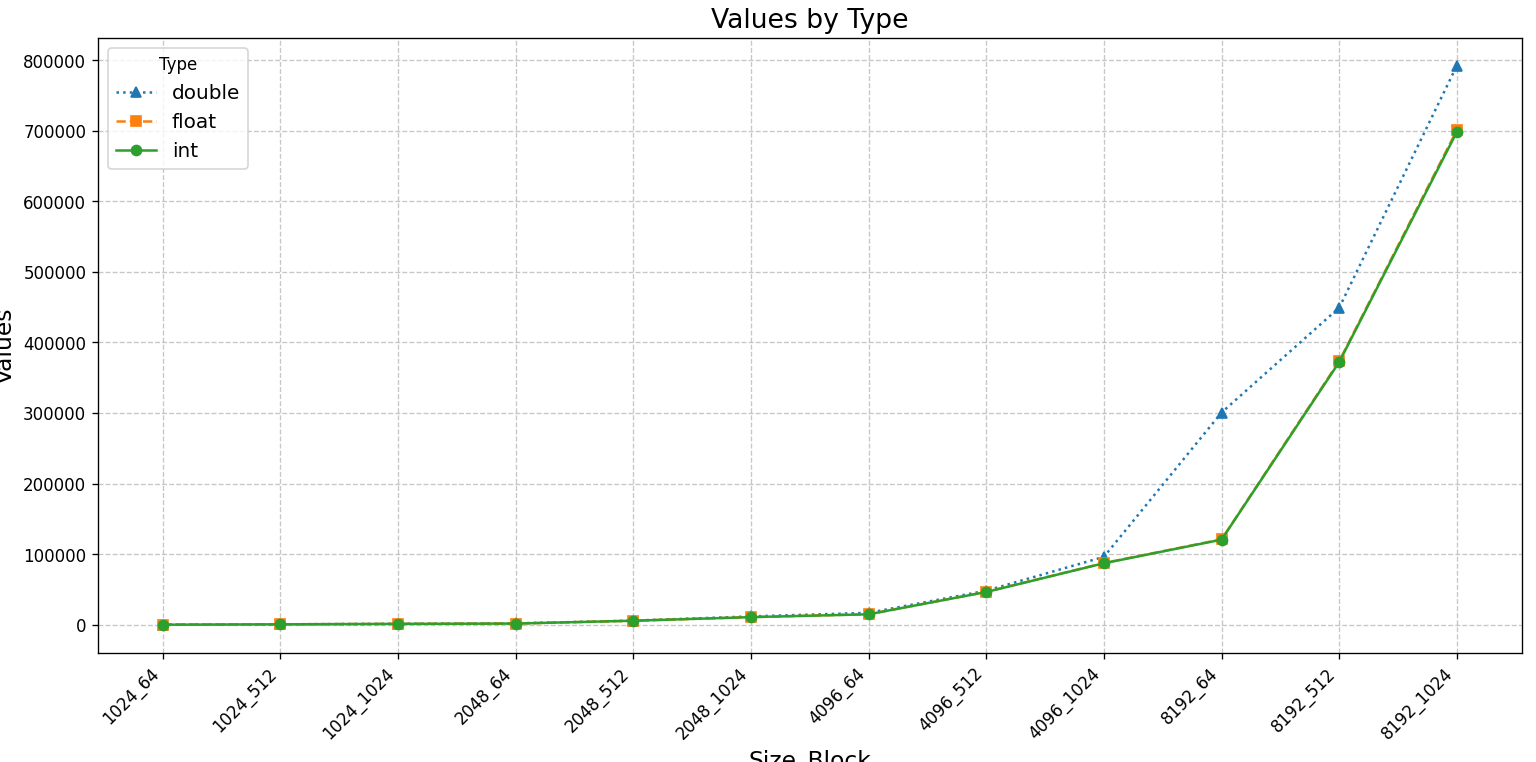
\includegraphics[width=0.8\textwidth]{4.png}
\end{figure}

As experimented the increase of size in int to float did not affect it to much that this may be because of the little difference in their sizes.


\section{BFS vs DFS Schemes}
Breadth-First Search (BFS) and Depth-First Search (DFS) schemes in CUDA.

\begin{figure}[h!]
    \centering
    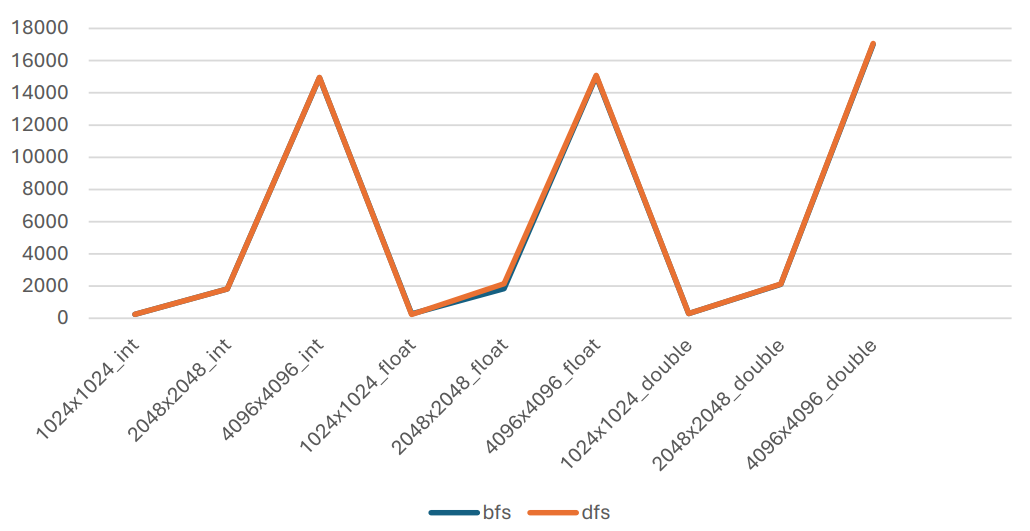
\includegraphics[width=0.8\textwidth]{5.png}
\end{figure}

As above the difference is negligible because new GPUs have more than one worker queue so the DFS call or BFS call won’t affect the pipe lining performance and parallelism can be done in every moments.


\section{cudaMalloc vs cudaMallocManaged}

I analyzed the performance difference between cudaMalloc (explicit memory allocation 
on the device) and cudaMallocManaged (Unified Memory).



\subsection{cudaMalloc:}

\\• Requires explicit memory management, including cudaMemcpy calls to transfer data between host and device. \\
\\• Offers higher performance for applications with predictable memory access patterns due to reduced runtime overhead. \\


\subsection{cudaMallocManaged:}

\\• Provides Unified Memory, simplifying memory management by automatically handling data movement. \\
\\• May introduce performance overhead due to page migration between host and device. \\


\subsection{Plot and Results:}

cudaMalloc is faster due to less runtime overhead and where cudaMallocManaged simplifies code development at the cost of some performance.


\begin{figure}[h!]
    \centering
    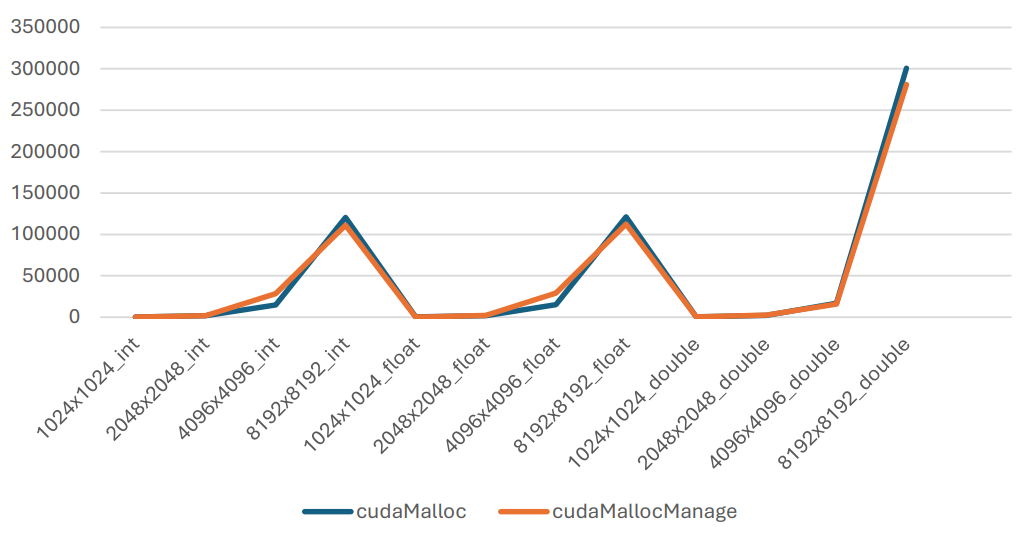
\includegraphics[width=0.8\textwidth]{6.png}
\end{figure}

\end{document}
